\documentclass{beamer}
\usepackage{textcomp}

\usetheme{Rochester}
\usecolortheme{crane}

\definecolor{umber}{HTML}{A3C9F4}
\definecolor{light}{HTML}{DBECFF}

\setbeamercolor{frametitle}{fg=black, bg=umber}

\setbeamercolor{block body example}{bg=light}
\setbeamercolor{block title example}{bg=umber}


\setbeamercolor{frametitle}{fg=black}
\setbeamercolor{title}{fg=black, bg=umber}

\begin{document}

  \title[Crisis] % (optional, only for long titles)
  {Migration and Segregation in Three Dimensional Cellular Co-cultures}
  \subtitle{Role of Differential Cell Adhesion and Elasticity}
  \author[Author, Kolbman] % (optional, for multiple authors)
  {Dan Kolbman\\Mentor: Moumita Das}
  \date[2014]
  {Capstone Preparation, Spring 2014}
  \subject{info}


  \frame{\titlepage}
  
  % BACKGROUND %
  \begin{frame}
    \frametitle{Background}
    \framesubtitle{Behavior of cancer cells}
    
    \begin{itemize}
    \item Cancer cells are mechanically softer than healthy cells of the same tissue type. 
    (Lee et al. Biophysical Journal 2012).
    \item Cancer cells show much less cell-cell adhesion than non-cancerous cells  due to deficiency of the protein E-cadherin. 
    (Cukierman et al., Science 2001)
    \item Cancer cells move more quickly in populations of healthy cells in 2D co-cultures. 
    (Lee et al, Biophysical Journal 2012, Butcher et al. unpublished).
    \item Cells move at different rates in $2D$ than in $3D$.
    (Cukierman et al., Science 2001)
    \item Cells move differently when confined in an extracellular matrix (ECM). 
    (Doyle et al., J. Cell Biol. 2009)       
    \end{itemize}
    \vfill
    
  \end{frame}  
  
  
   % MOTIVATION %
  \begin{frame}
    \frametitle{Motivation}
    \framesubtitle{New experimental data}
    
    \begin{enumerate}
    \item New experiments and techniques are becoming available to observe cellular co-cultures in $3D$
    
    \item Little theoretical understanding of biomechanics and biophysics of cell co-cultures existing in $3D$
    \end{enumerate}
    
    \vspace{0.5in}
    
	\center\emph{Can we propose a new model of cancer cell aggregation and migration in $3D$? \\
	Can we obtain insights from these results about the underlying physical mechanism of metastasis?}
    
    \vfill
    
  \end{frame}
    
  
  % MODEL %
  \begin{frame}
    \frametitle{The Model}
    Minimum Ingredients
    \begin{itemize}
    \item Binary system of colloids 
    \item Activity (self-driven forces due to ATP consumption)
    \item Cell deformability
    \item Cell-cell adhesion
    \item Confinement
    \item Surrounding extracellular matrix
    \end{itemize}
    
	\begin{exampleblock}{Over Damped Langevin Equation}
	$$\vec{F}(\vec{r _m}) - \gamma \frac{d\vec{r_m}}{dt} + \vec{\eta}(t) = 0$$
	\end{exampleblock}
	\begin{columns}[t]
    \column{.5\textwidth}
     $\vec{F}$ -- Total force on the cell \\
     $\gamma$ -- The damping coefficient \\
      $\vec{r_m}$ -- Particle position. \\
    \column{.5\textwidth}
    $\vec{\eta}$ -- Fluctuating force to approximate collisions with smaller particles \\
    \end{columns}
    
    \vfill
    
  \end{frame}
  
  % EXPERIMENTAL %
  \begin{frame}
    \frametitle{Experimental Conditions}
  	\begin{columns}[t] 
  	\column{0.3\textwidth}
  	\begin{figure}
  	  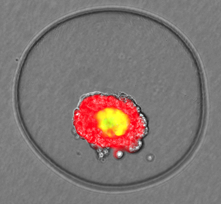
\includegraphics[width=1.0in]{minglin.png}
  	  \caption{Experimental Image (Minglin Ma, Mingming Wu)}
  	\end{figure}
    \column{.3\textwidth}
    \begin{figure}
      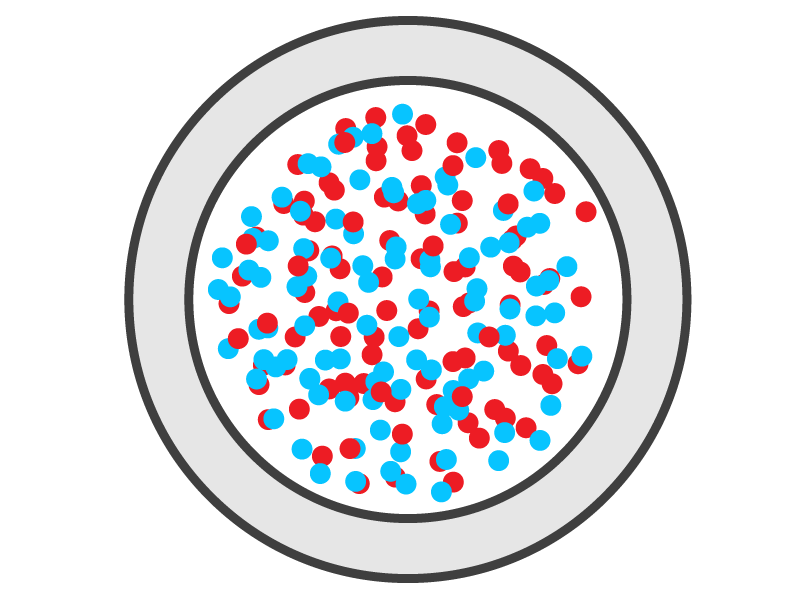
\includegraphics[width=1.25in]{Fig1.png}
      \caption{A capsule containing a cellular co-culture}
    \end{figure}
    \column{.3\textwidth}
    \begin{figure}
      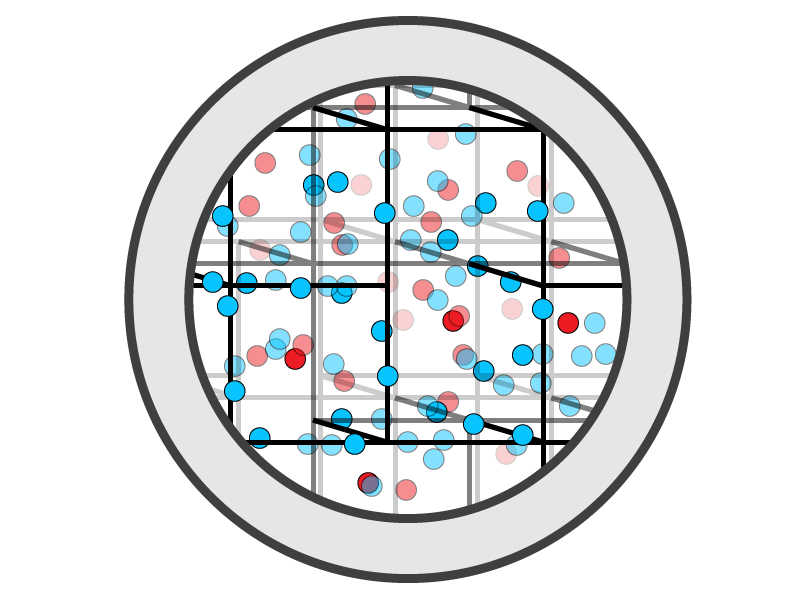
\includegraphics[width=1.25in]{Fig2.png}
      \caption{A capsule with a disordered matrix}
    \end{figure}
    \end{columns}
    
    Inner diameter -- $50-700$ \textmu m\\
    Outer diameter -- $400-7000$ \textmu m\\
	Cell diameter -- $\sim 10$ \textmu m\\
    
    \vfill
    
  \end{frame}
  
  % Timeline %
  \begin{frame}
    \frametitle{Timeline}
    
      {\bf Capstone I}
      \begin{itemize}\itemsep1pt \parskip0pt 
		\item Dynamics for One Species in $3D$, with boundary conditions (4 weeks).
		\item Binary system, with different stiffness (3 weeks)
		\item Differential cell-cell adhesion for the two cell types. (3 weeks) 
		\item Collect Data, Analyze Results (3 weeks)
		\item Examine physical and biological implications of results so far,
local conference, write paper, talk (2 weeks)\\

	  \end{itemize}
	  
  \end{frame}
  
  % TIMELINE %
  \begin{frame}
    \frametitle{Timeline}
  	
  	{\bf Capstone II}
	  \begin{itemize}\itemsep1pt \parskip0pt
	  	\item Apply experimental values to model, identify relevant regimes of parameters, compare results of model thus far with control experiments in collaboration with Drs. Wu and Ma (2 weeks) 
		\item Add extracellular matrix. (4 weeks)
		\item Add self propulsion forces.(2 weeks)
		\item Obtain results and analyze and interpreted  data. (2 weeks)
		\item Attend March Meeting and present results (1 week)
		\item Calculate phase diagram of aggregation and migration speed. (2 weeks)
		\item Compare final results with experiments write paper, give talk. (2 weeks)
		
	  \end{itemize}
    
    \vfill
    
  \end{frame}
  
  % THANKS %
  \begin{frame}
    \frametitle{Thanks}
  	\begin{center}
  	 You!! \\
     Dr. Moumita Das\\ Julian Butcher\\ Dr. Mingming Wu and Dr. Minglin Ma\\
     Dr. Linda Barton and Capstone Committee \\

	\vspace{0.3in}     
     
     Budget: Textbooks, articles (\$100), Software (\$50)
    
  	\end{center}
  	  
    \vfill
    
  \end{frame}

\end{document}
